\subsection{Overview}

\begin{figure}
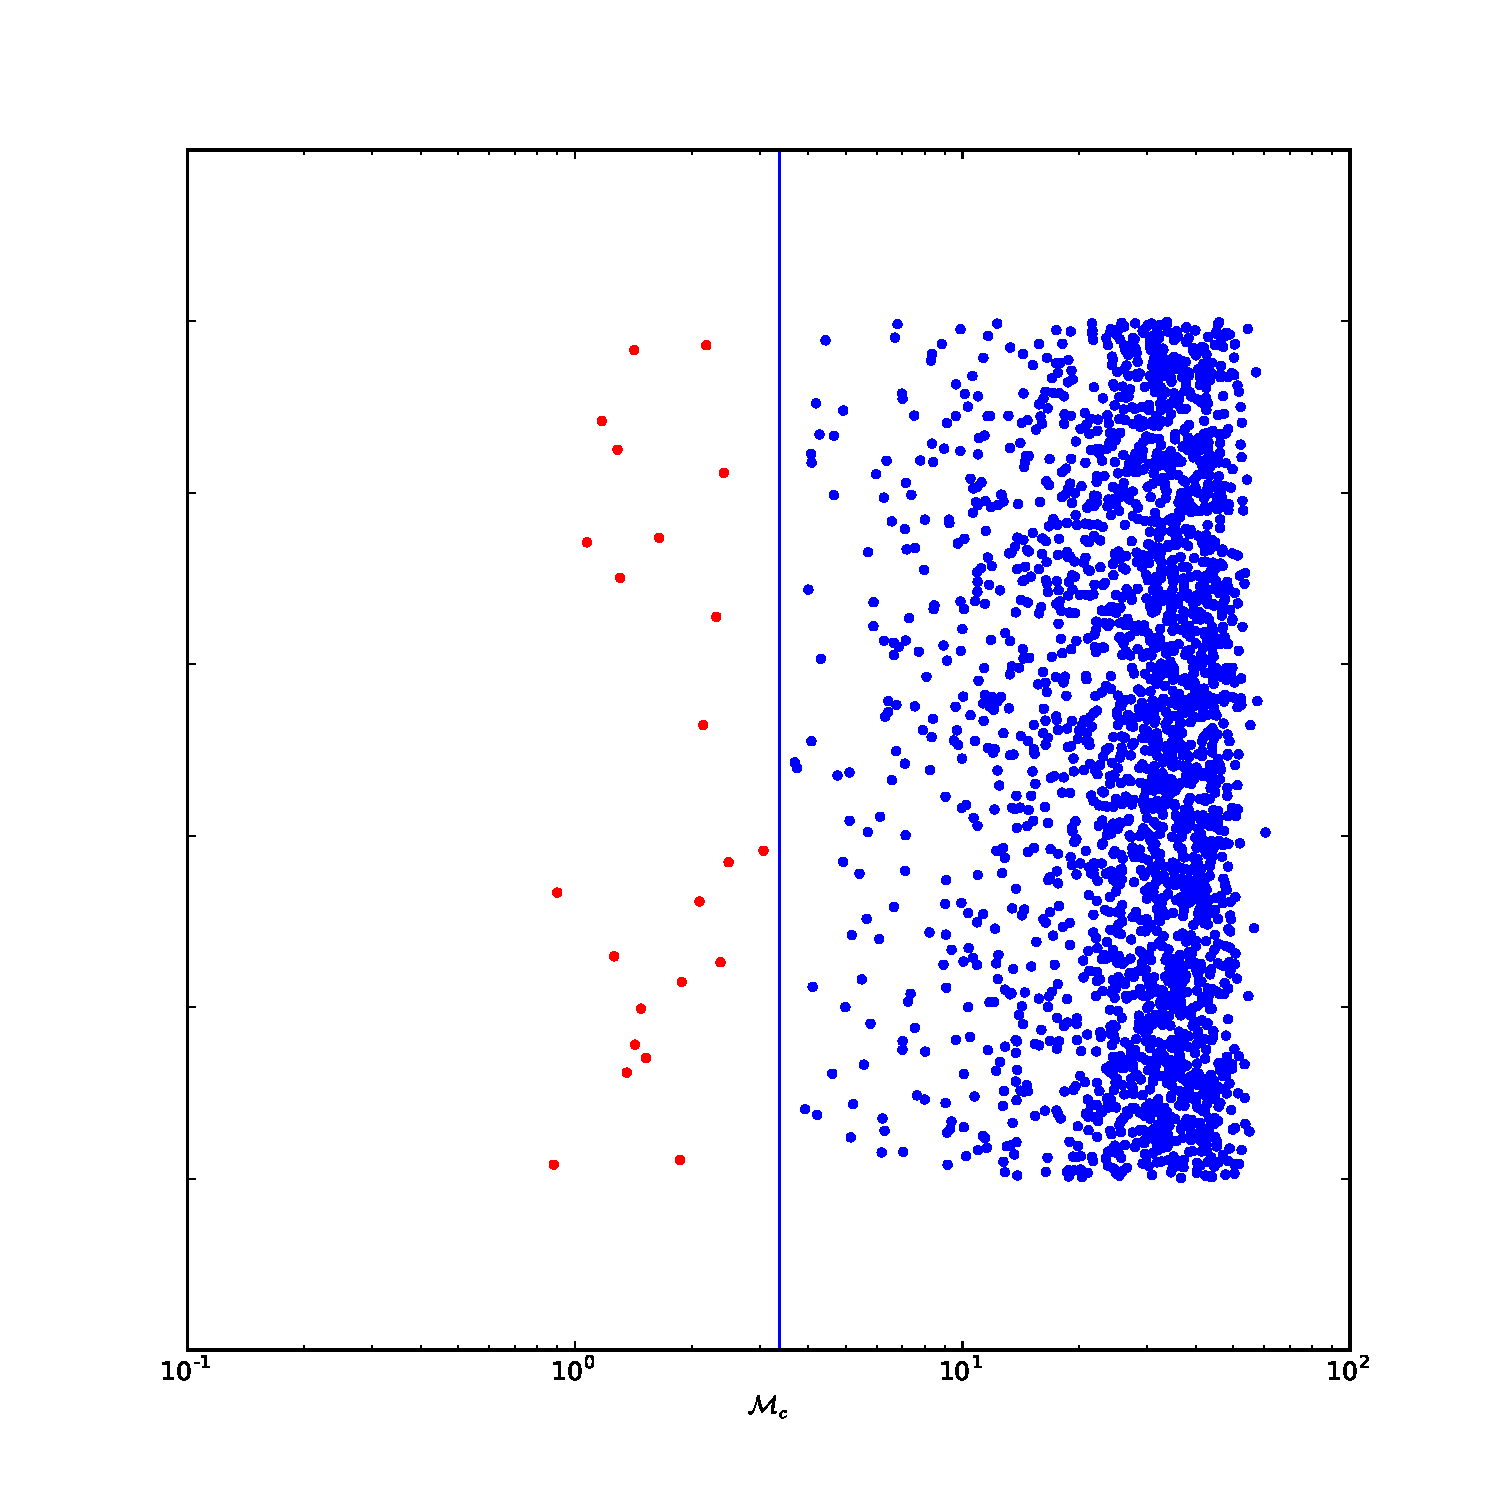
\includegraphics[width=\columnwidth]{output/jake/classifier_half.pdf}
\caption{This shows the first half of the data with the same two groups as before. The vertical line indicates the division between the two groups.}
\label{fig:half}
\end{figure}
\begin{figure}
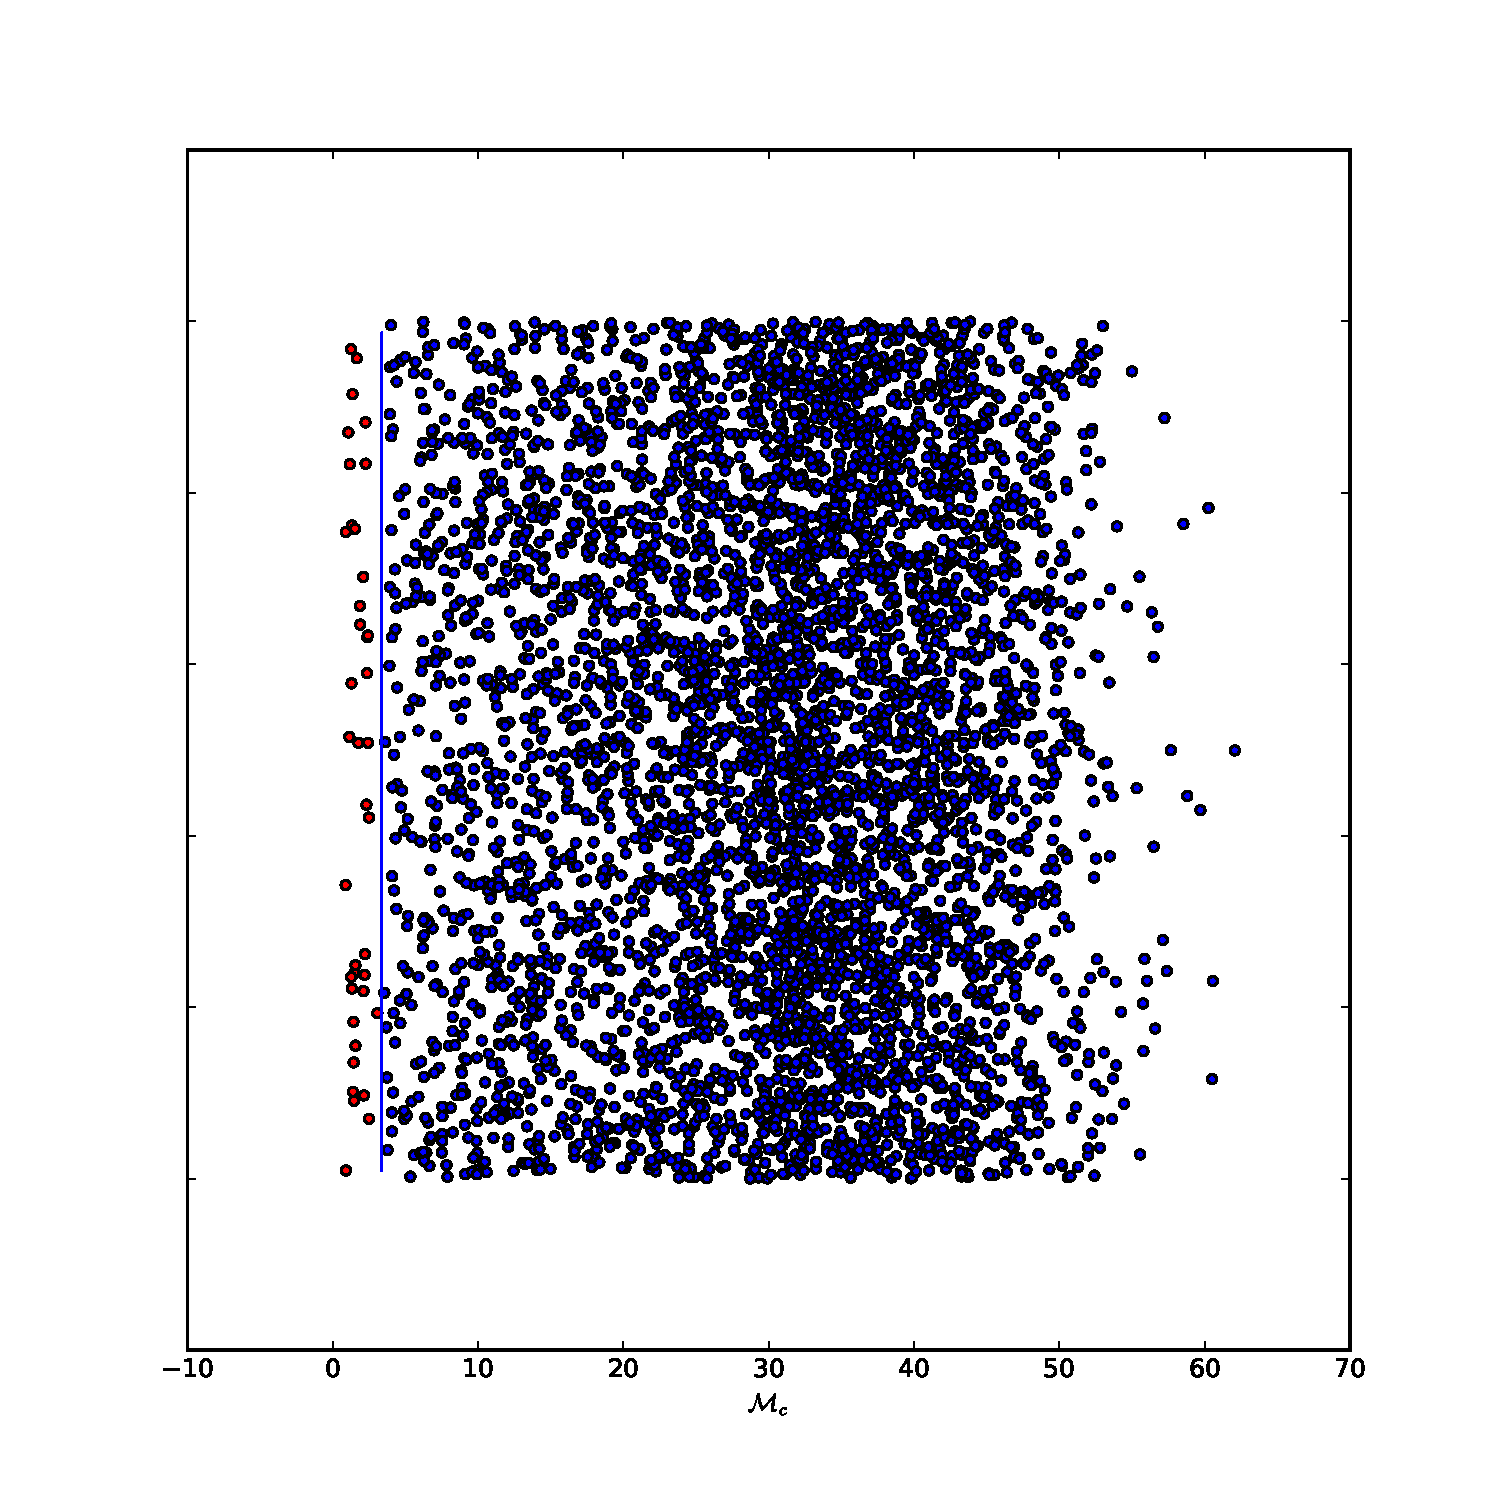
\includegraphics[width=\columnwidth]{output/jake/classifier_all.pdf}
\caption{This shows the full set of the data with the dividing line trained by half the data.}
\label{fig:all}
\end{figure}

The GW observatory, the Laser Interferometer Gravitational Wave Observatory (LIGO), can provide very rapid mass estimates of candidate GW events. Since most of these detections are mostly binary black holes and electromagnetic followup is extremely expensive, only a few events can be followed up. We have therefore trained a classifier to determine if an event will have a electromagnetic followup. We trained this classifier on the first half of the data. We simply took the mid-way point betweewn the maximum chirp mass for the electromagnetic counterpart group and the other group. This is shown in Figure \ref{fig:half}. This was then used on the whole dataset as shown in Figure \ref{fig:all}.

\subsection{Method}
The classifier was constructed simply by taking the minimum chirp mass event of the other group (no electromagnetic counterparts) and the maximum chirp mass event of the electromagnetic counterpart group and finding the distance between those two events. This trained for the first half of the dataset. The result can be seen in Figure \ref{fig:half}; the vertical line represents half the distance between the maximum chirp mass of the electromagnetic counterpart group and the other group.

